\documentclass[english,11pt,usenames,dvipsnames]{beamer}

\DeclareMathOperator{\Cov}{Cov}
\DeclareMathOperator{\Var}{Var}
\DeclareMathOperator{\E}{\mathbb{E}}
\DeclareMathOperator{\Proba}{\mathbb{P}}

\newcommand{\Covb}[2]{\ensuremath{\Cov\!\left[#1,#2\right]}}
\newcommand{\Eb}[1]{\ensuremath{\E\!\left[#1\right]}}
\newcommand{\Pb}[1]{\ensuremath{\Proba\!\left[#1\right]}}
\newcommand{\Varb}[1]{\ensuremath{\Var\!\left[#1\right]}}

% norm
\newcommand{\norm}[1]{\| #1 \|}

\newcommand{\indep}{\rotatebox[origin=c]{90}{$\models$}}





\usepackage{mathptmx,amsmath,amssymb,graphicx,bibentry,bbm,babel,ragged2e}

\makeatletter

\newcommand{\noun}[1]{\textsc{#1}}
\newcommand{\jitem}[1]{\item \begin{justify} #1 \end{justify} \vfill{}}
\newcommand{\sframe}[2]{\frame{\frametitle{#1} #2}}

\newenvironment{centercolumns}{\begin{columns}[c]}{\end{columns}}
%\newenvironment{jitem}{\begin{justify}\begin{itemize}}{\end{itemize}\end{justify}}

\usetheme{Warsaw}
\setbeamertemplate{footline}[text line]{}
\setbeamercolor{structure}{fg=purple!50!blue, bg=purple!50!blue}

\setbeamersize{text margin left=15pt,text margin right=15pt}

\setbeamercovered{transparent}

\setbeamertemplate{headline}{}
\setbeamertemplate{footline}[frame number]
\setbeamertemplate{navigation symbols}{}

\@ifundefined{showcaptionsetup}{}{%
 \PassOptionsToPackage{caption=false}{subfig}}
\usepackage{subfig}

\usepackage[utf8]{inputenc}
\usepackage[T1]{fontenc}


\usepackage{tikz}

\usepackage{multirow}

\usepackage{mdframed}

%\usepackage[usenames,dvipsnames]{pstricks}
%\usepackage{auto-pst-pdf}


%\usepackage[dvipsnames]{xcolor}

\usepackage{threeparttable}


\makeatother

\begin{document}


\title{Linking Microsimulation and LUTI models}

%\author{J.~Raimbault$^{1,2,3}$\\
%\texttt{juste.raimbault@iscpif.fr}
%}


%\institute{$^{1}$UPS CNRS 3611 ISC-PIF\\
%$^{2}$CASA, UCL\\
%$^{3}$UMR CNRS 8504 G{\'e}ographie-cit{\'e}s
%}

\date{11/06/2019}

\frame{\maketitle}



%\section{Introduction}


\sframe{Context}{

}

\sframe{Outline}{
\tableofcontents
}

\section{Literature mapping}
% global overview with citation maps 
% (different use of microsim)


\sframe{Citation network analysis}{

\justify

 % - very different approaches with same name ?
 % - potential/relevance to couple approaches ?

 \begin{itemize}
 	\item Urban modeling in general very broad on models used and how to name/describe them
 	\item What are existing existing/potential connections between approaches?
 \end{itemize}
 
 \bigskip

 $\rightarrow$ \textit{a systematic review and citation network exploration around our main entries (microsimulation and luti)}

 \medskip
 
 Currently :
 
 \begin{itemize}
 \item Extended/rewrote a bibliographic data collection and management library (java) to get citation data from google scholar
 \item 
 \end{itemize}
 
 
 

}

\sframe{Coverage of the citation network}{
  
  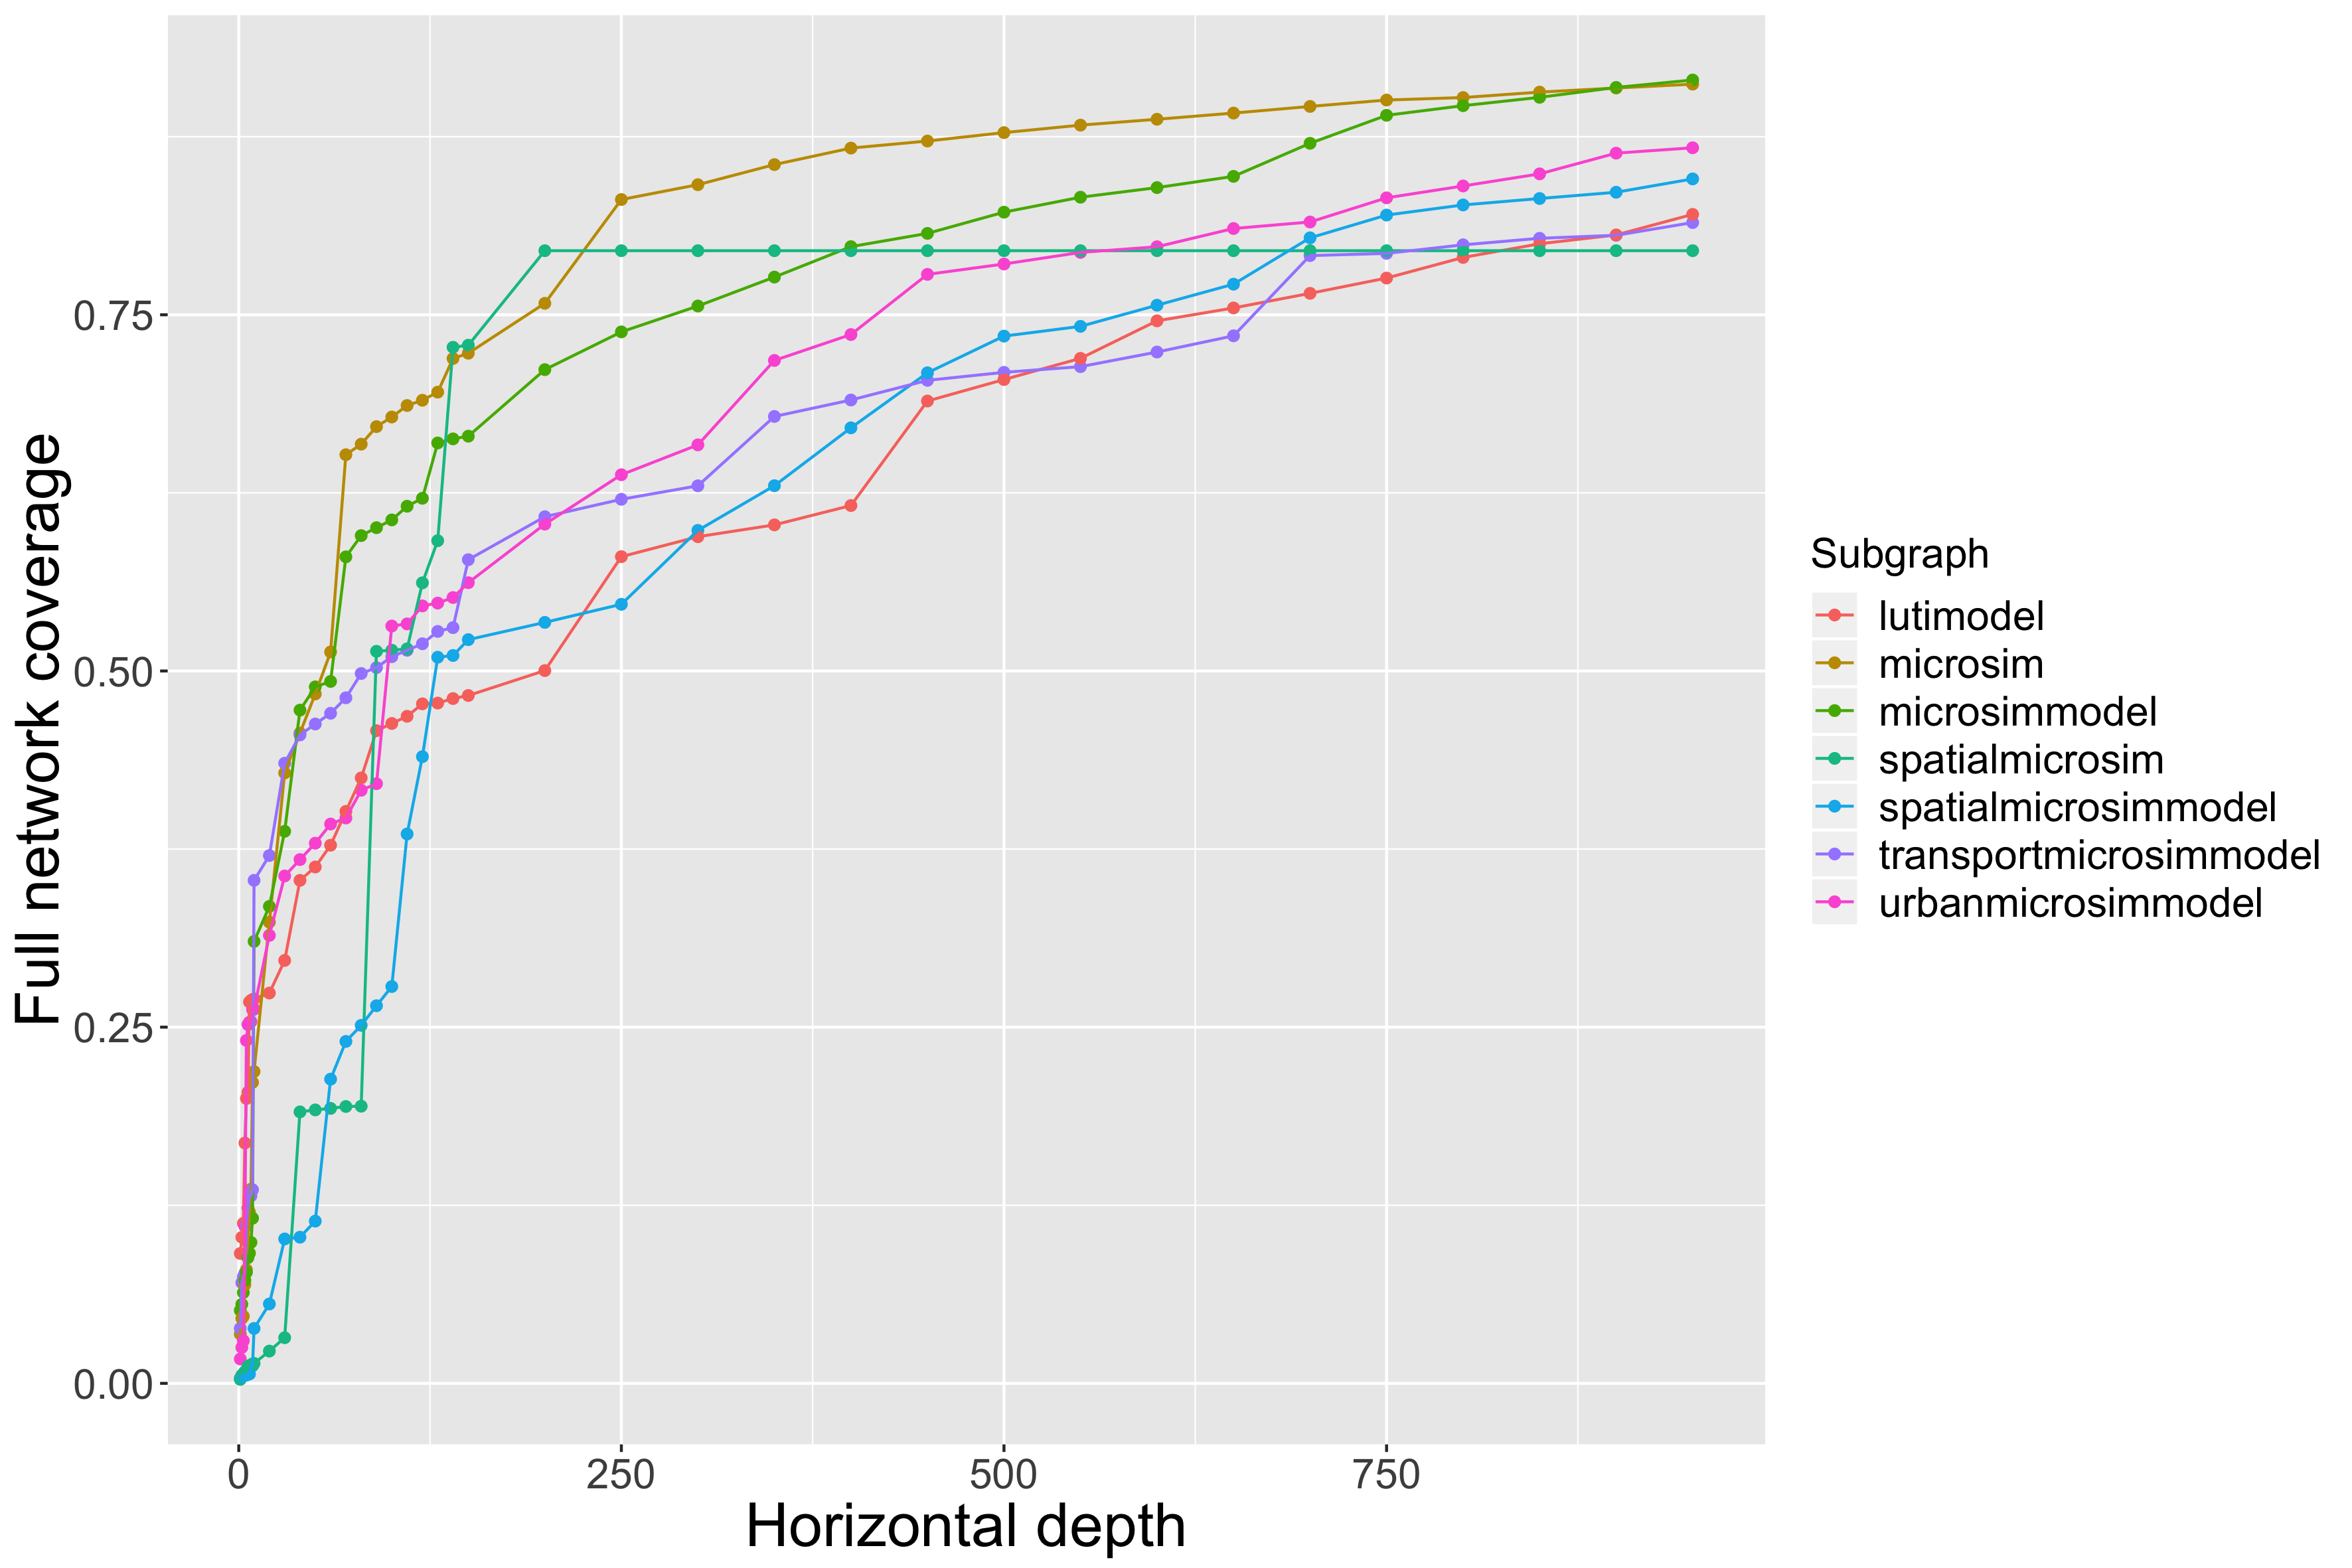
\includegraphics[width=\textwidth]{figures/coverage_subnws}
  
}

\sframe{Citation network}{

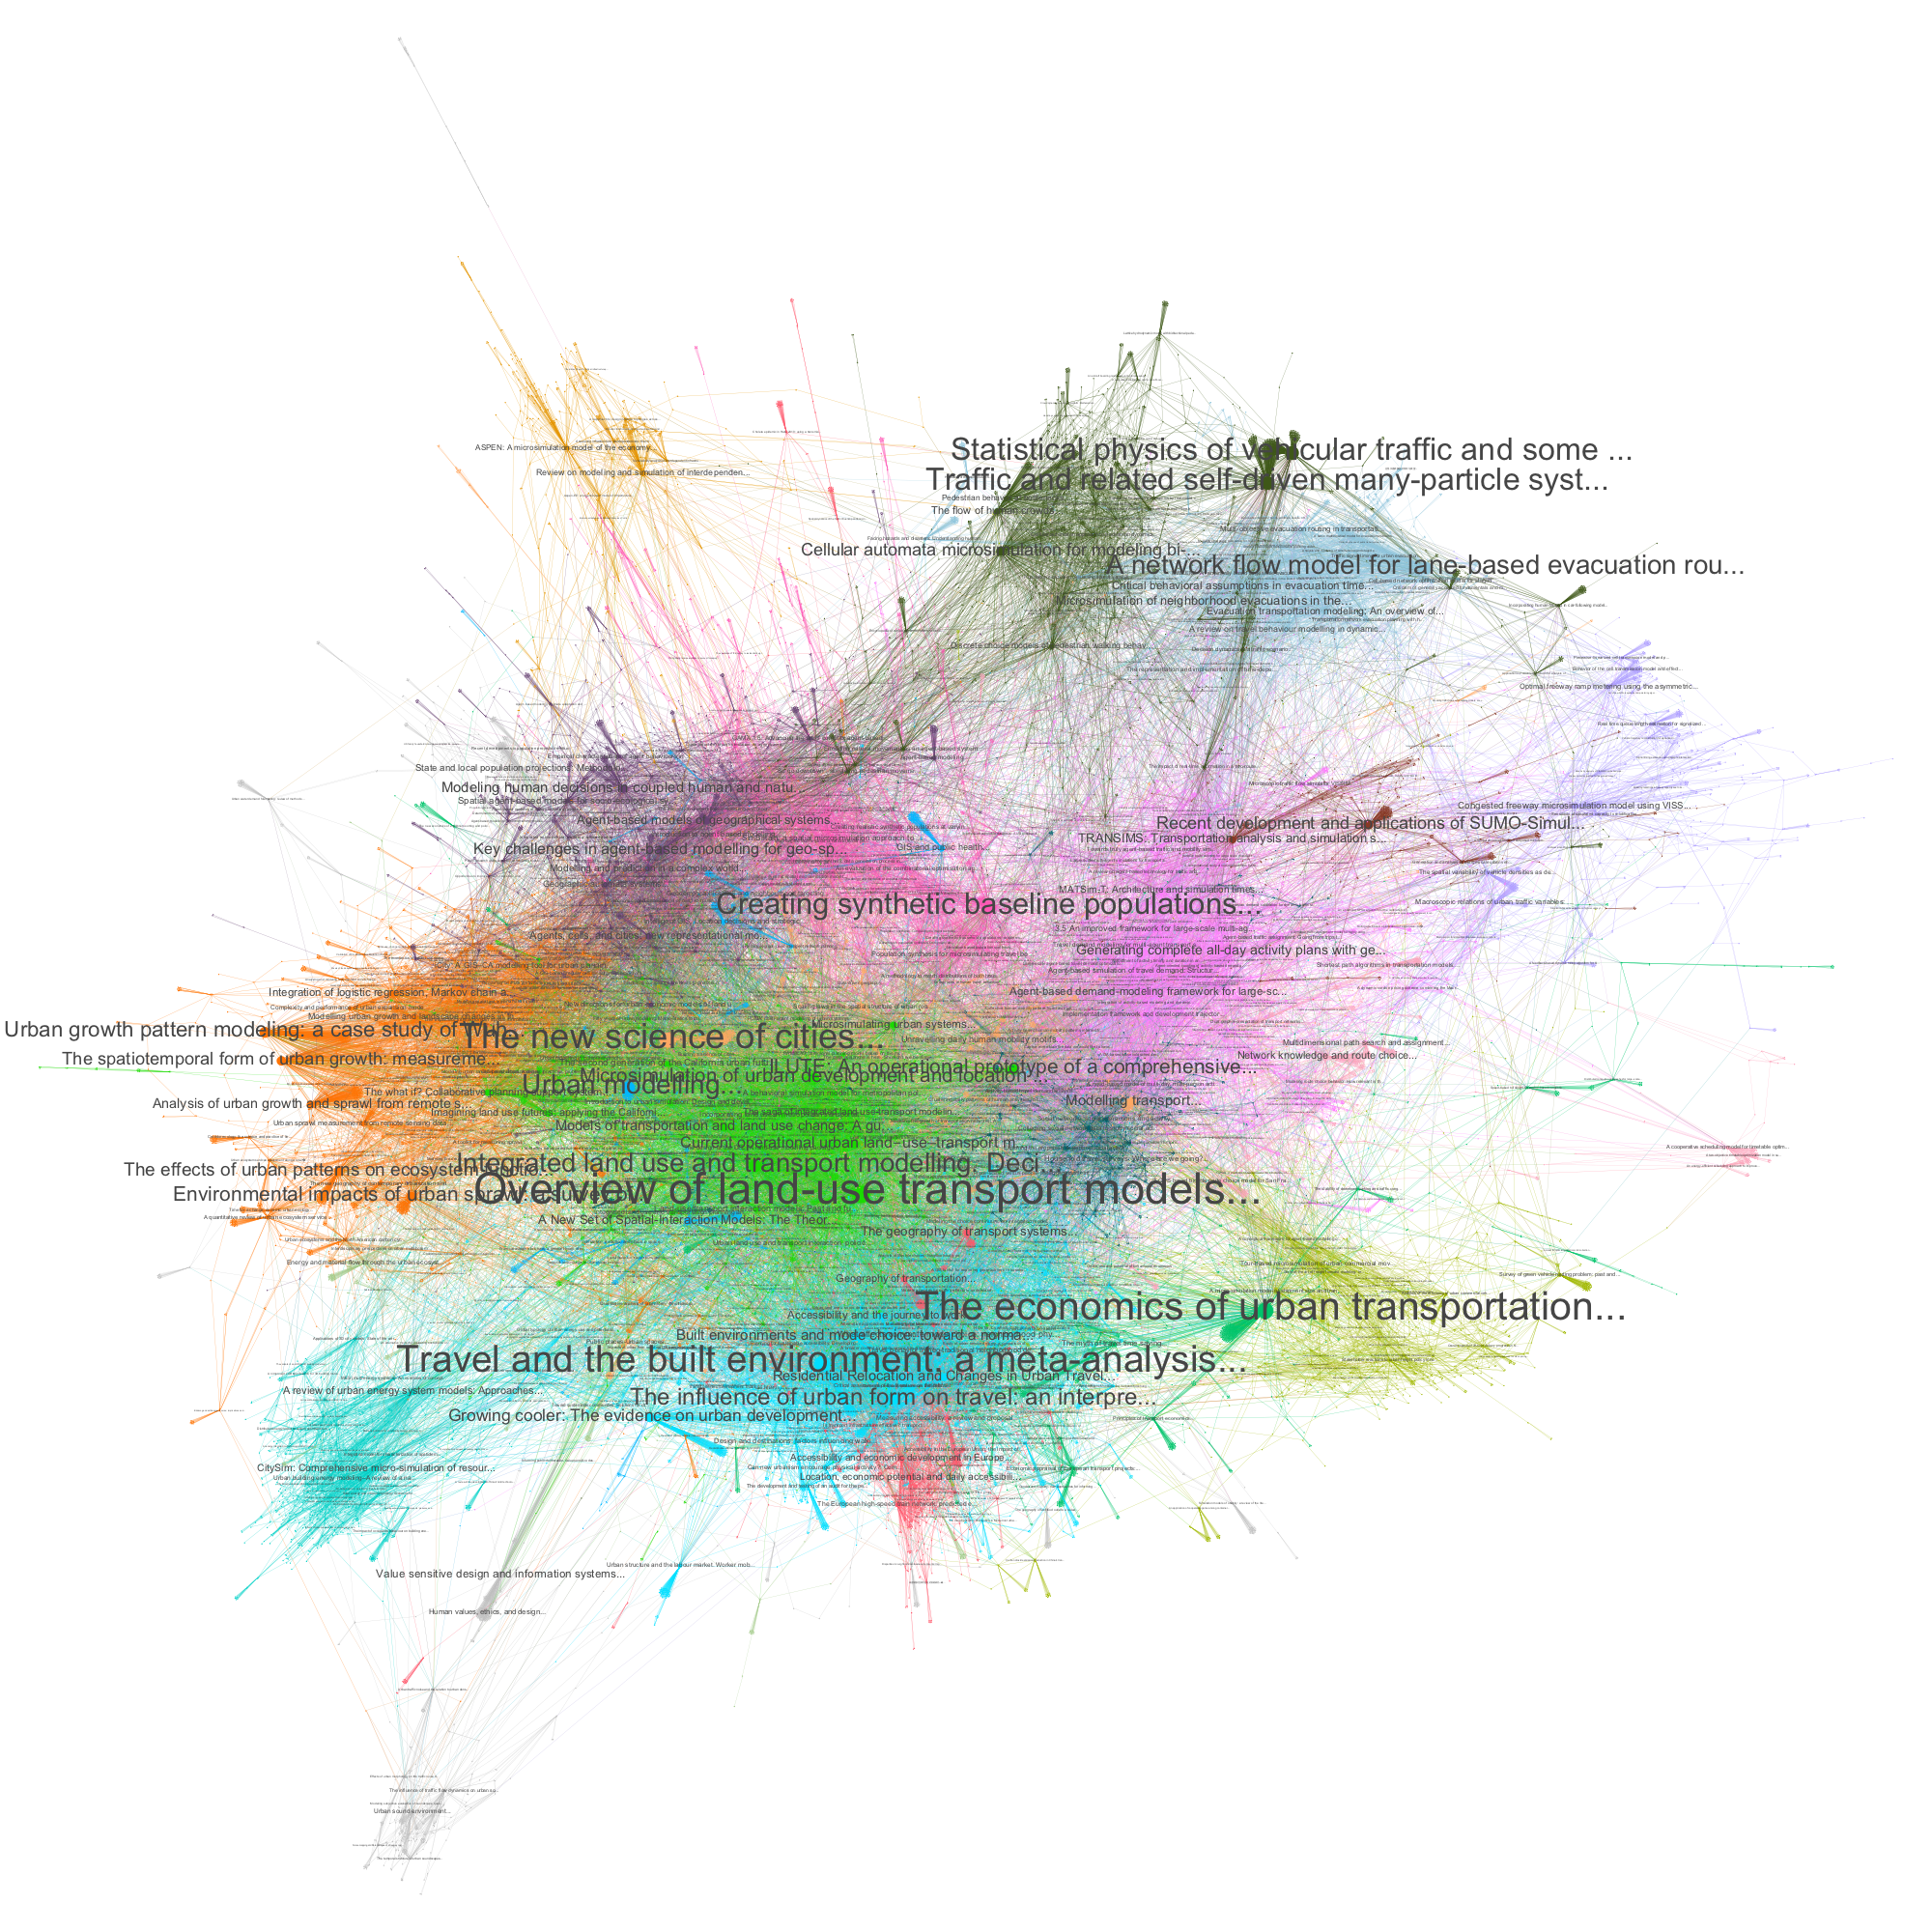
\includegraphics[width=\textwidth]{figures/core_hdepth3_filtered_LOWRES.png}

}

\sframe{Core communities}{

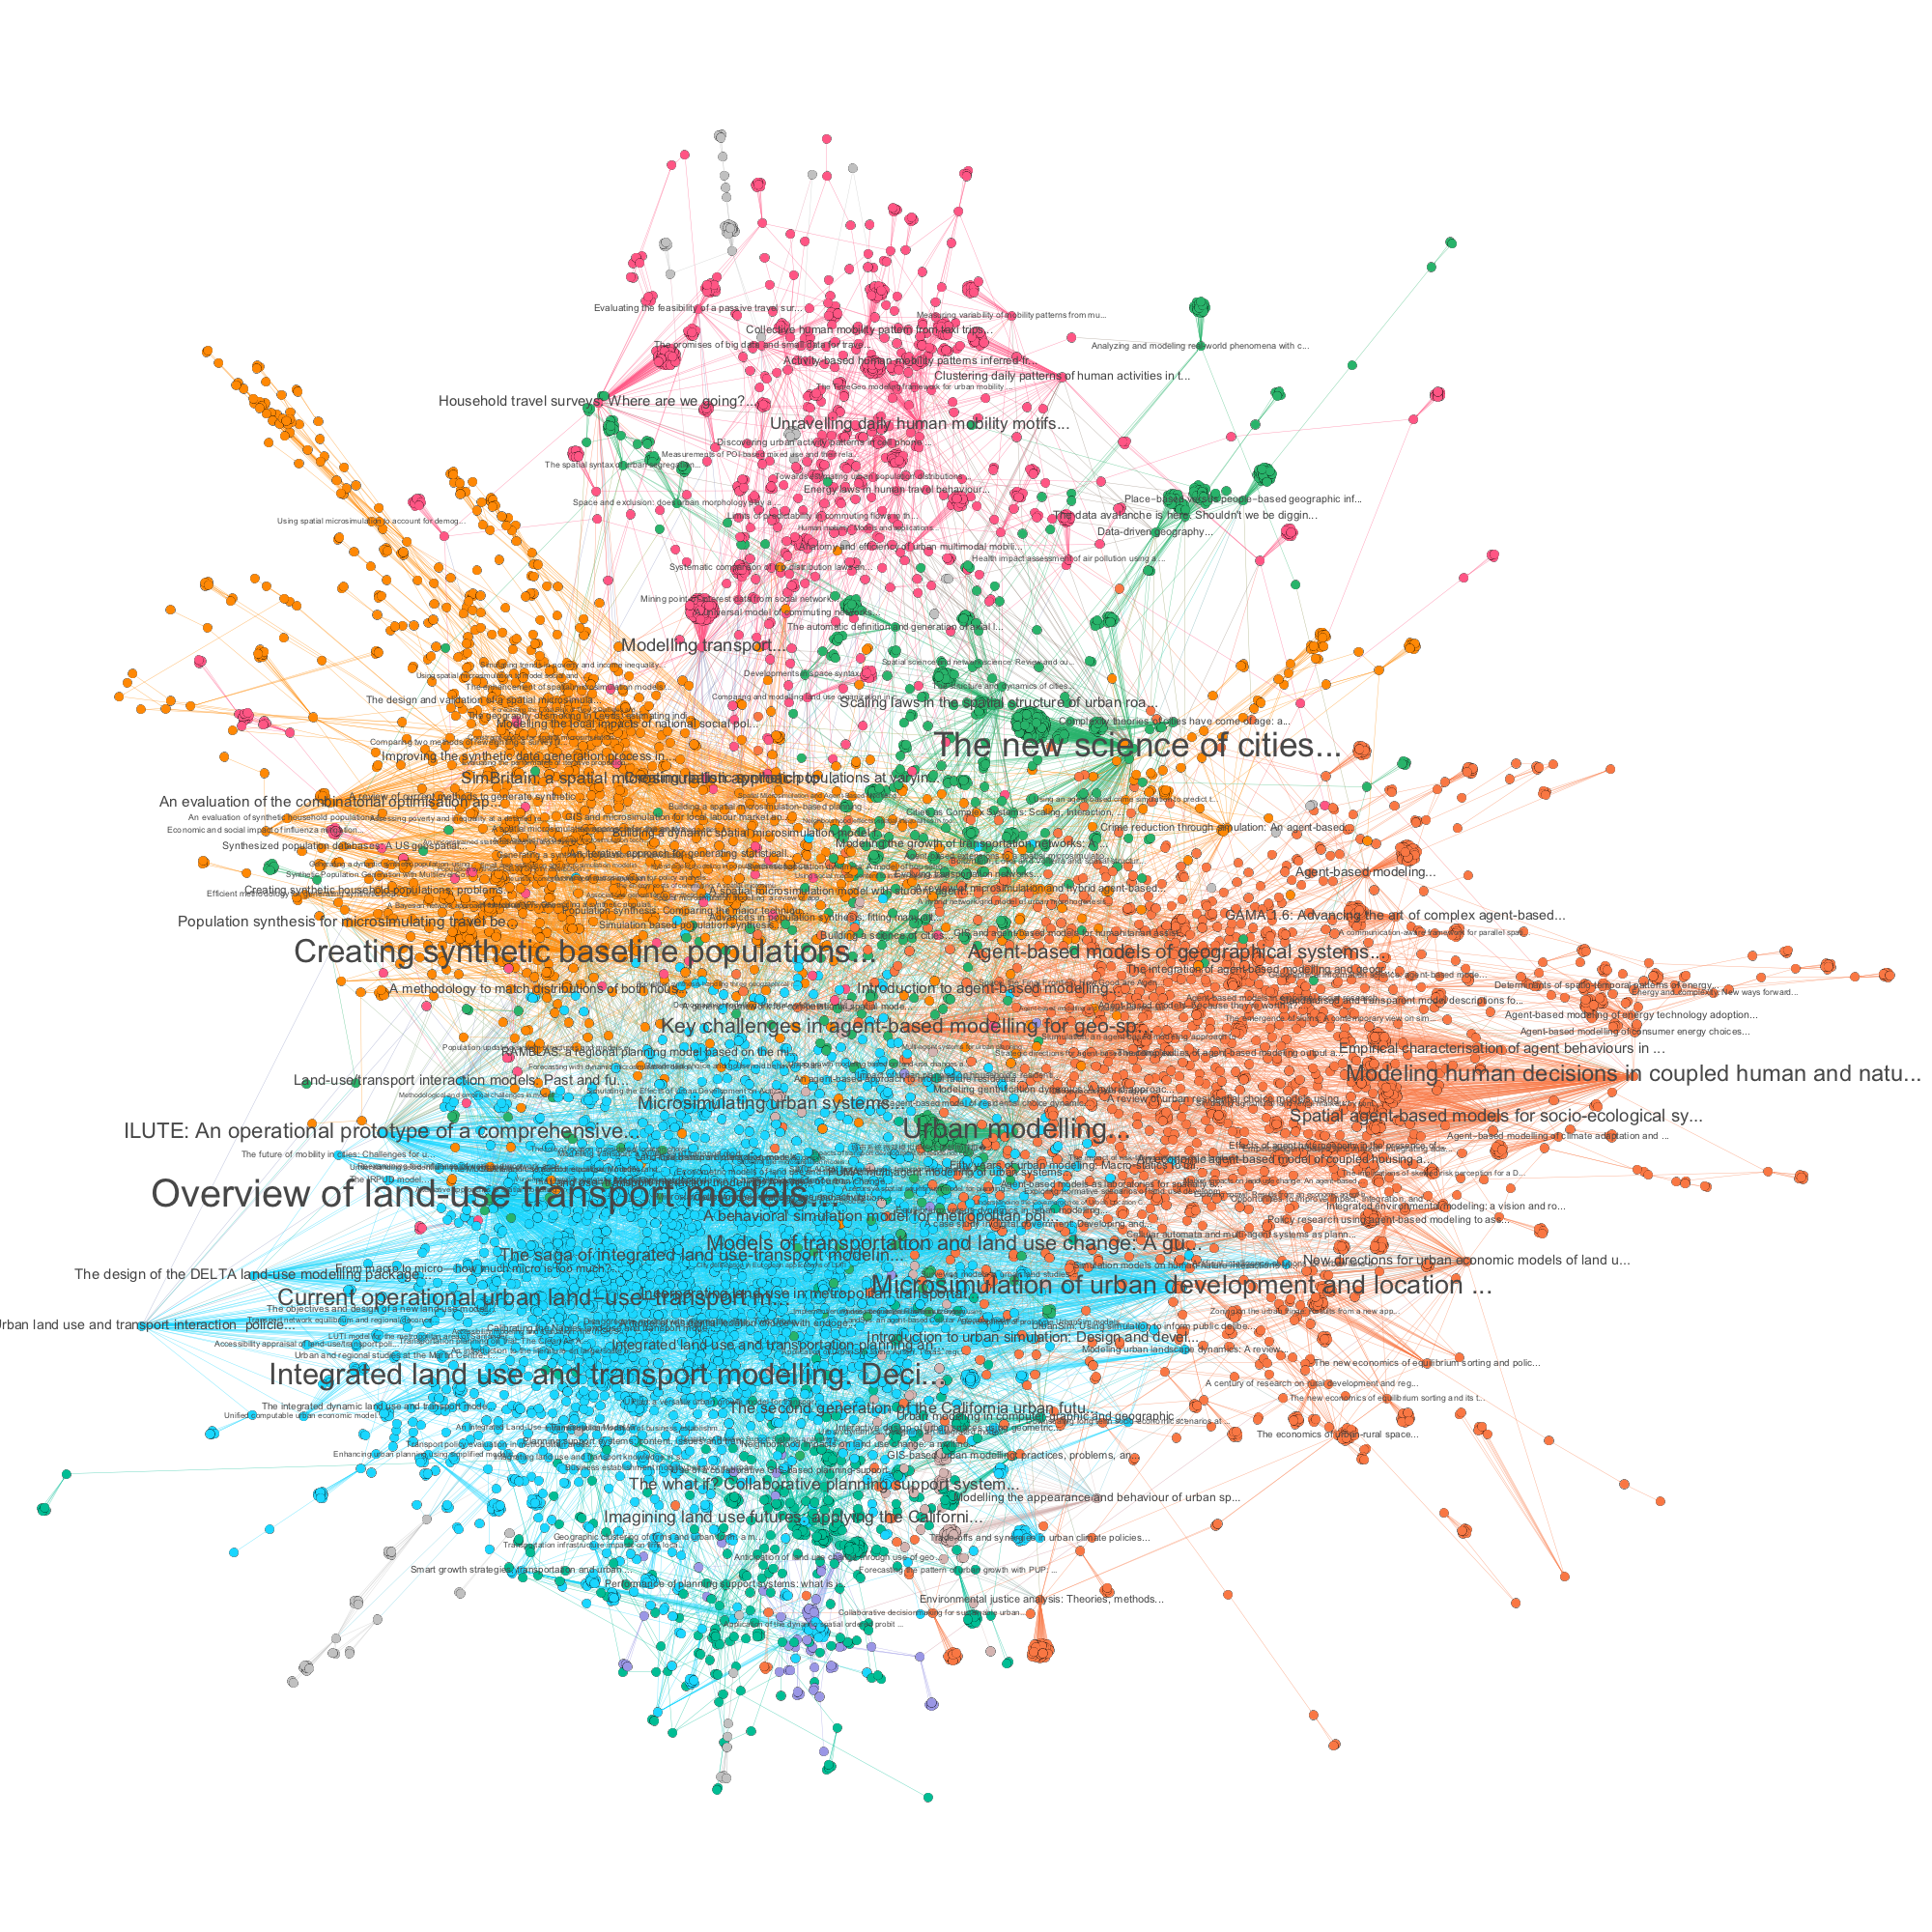
\includegraphics[width=\textwidth]{figures/core_hdepth3_filtered_targeted_LOWRES.png}

}



\section{Specific definitions}



\section{Description of SPENSER}

\sframe{General purpose}{

  Individual and household-level simulation of population

  $\rightarrow$ test policies and scenarios at the UK-level
  
  \medskip
  
  Modules:
  
  \begin{itemize}
  	\item Synthetic population generator %(Iterative Prop Fitting)
  	\item Dynamic micro-simulation library
  	\item Simim, spatial interaction library
  \end{itemize}
  
}

\sframe{Synthetic population generation}{

}

\sframe{Dynamic microsimulation}{

}

\sframe{Spatial interactions}{

}

\sframe{Technical aspects}{

	% python + cpp // quant developed by Maarten using simim library


}



\section{Coupling QUANT and SPENSER: prospects}

% -> roadmap, incl sensitivity analysis

\sframe{Comparison of properties}{

%%%%%%%%%%%%
\begin{table}
\begin{threeparttable}
	%\caption{Main characteristics of QUANT and MOSES models.}\label{tab:comparison}
	\centering
	\begin{tabular}{|c|p{6cm}|p{6cm}|}
	%\hrule
	& QUANT & SPENSER \\
	%\hrule
Time scale & 10 years $^{\ast 1}$ & 30 years \\
Spatial scale & UK & UK \\
Spatial resolution & MSOA & Ward \\
Agent granularity & Aggregated counts & individual level \\
Static/Dynamic & Equilibrium (static) & Dynamic $^{\ast 2}$ \\
Randomness & Deterministic & Monte-Carlo simulations \\
Process: Transportation & 3 modes $^{\ast 3}$ & NA \\
Process: Economic activities & Accessibility-based relocations & NA \\
Process: Demographics & NA & Data-driven $^{\ast 4}$ \\
Process: Migration flows & Accessibility-based relocations & Data-driven \\
%\hrule
	\end{tabular}
	\begin{tablenotes}
      \small
      \item $^{\ast 1}$ stylized time scale of metropolitan relocations \cite{wegener2004land}
      \item $^{\ast 2}$ model structure is however stationary - this is an important issue for a possible application to 2070
      \item $^{\ast 3}$ discrete choice for transportation mode is not implemented in QUANT 
      \item $^{\ast 4}$ probabilities of basic demographic events (ageing, mortality, fertility, household formation, health, migration) are computed from data
    \end{tablenotes}
	\end{threeparttable}
\end{table}
%%%%%%%%%%%%


}

\sframe{Alternatives for coupling}{

% \item Weak coupling Luti $\rightarrow$ microsimulation: using sequentially outputs of Quant as inputs of Moses. For example, evaluating a new transportation scenario will provide predictions for new populations, employments and commuting flows. Distributing the synthetic population and its movements conditionally to this new distribution (respecting reasonably some statistical properties of the original data, what may pose difficult synthetic data generation problems), and running the microsimulation model with this new parametrization, could provide micro-based measures of the impact of the new transportation line (e.g. exposure to pollution, access to health facilities, segregation, etc.). In that case, it does not seem to make much sense to use the aggregated prediction of the microsimulation model, since the uncertainty on input data will be high as a output of the upstream model (``\textit{garbage in-garbage out}''), and the coupled model has a prospective and scenario-testing function.
%\item Weak coupling Microsimulation $\rightarrow$ Luti: the other way around, population projections obtained with microsimulation, which should be more precise than relocations by Quant (assuming that the system remains stationary and that exogenous effects are reasonably included), can be used as an input of the Quant model, in order to apply it in future times when for example planning long term infrastructure projects. More accurate future populations will provide more accurate generalized accessibility projections given or not some modification of the transportation network. The question answered and model function would also be territorial prospective. %(\textit{Open question : how do model functions in the sense of the typology of \cite{varenne2017theories} evolve during model coupling, do some typical patterns exist or is it case/scale specific ? Given a ``strength'' of models (a partial order on a subset of models given some objectives), are there patterns on the strength of the coupled model ?})
%\item Both previous proposition make sense assuming large approximations and assumptions. However, assuming in the first case that population statistical properties remain similar after urban changes is not accurate, as the composition of population or their behavior may drastically change. In the second case, assuming that population projections do not depend much on the changes in the accessibility landscape is also not accurate. A strong coupling Microsimulation $\rightarrow$ Luti, in a sense a co-evolutive model between  demographic dynamics and dynamics of accessibility in terms of transportation, population and jobs, would object to these two inaccuracies and in theory be more appropriate. It would provide both applications, i.e. population exposure impacts of transport and land-use scenarios, but also accurate projections and planning. This being said, this approach must be taken with caution. Very few co-evolution models of territorial systems (whatever the objects studied) do exist in the literature, and the problem remains relatively opened methodologically, theoretically and empirically (e.g. \cite{raimbault2018modeling} extended the city system model of \cite{raimbault2018indirect} to provide a co-evolution model between transportation networks and territories at the macro-scale, which although very novel as such kind of models remains very simple and highly limited). For example, one can use Quant population dynamics to constraint microsimulation probabilities at fixed time steps, or one can on the contrary use microsimulation outputs as additional exogenous constraints for Quant which will be useful to redistribute employments and a given transportation scenario on a long time period. Many different coupling choices must be more thoroughly listed, studied and possibly compared. In that sense, building a strongly coupled model is similar to constructing a new model.


\begin{itemize}
	\item Weak coupling Luti $\rightarrow$ microsimulation
	\item Weak coupling Microsimulation $\rightarrow$ Luti
	\item Strong coupling
\end{itemize}


\medskip

$\rightarrow$ technically achieve one weak is a first requirement ; also requieres sensitivity analysis

$\rightarrow$ strong coupling can be seen as building a new model


}



\section{Sensitivity analysis}

% incl description of OpenMOLE


\sframe{Sensitivity analysis of SPENSER}{
 
  % validation of spatial interaction module
  
 
}

\sframe{Sensitivity analysis of QUANT}{

}


\sframe{Computational experiments using OpenMOLE}{

}

\sframe{Running OpenMOLE on DAFNI}{

}


\sframe{Conclusion: roadmap}{

}




%%%%%%%%%%%%%%%%%%%%%
\begin{frame}[allowframebreaks]
\frametitle{References}
\bibliographystyle{apalike}
\bibliography{biblio}
\end{frame}
%%%%%%%%%%%%%%%%%%%%%%%%%%%%










\end{document}







